\documentclass[20pt,margin=1in,innermargin=-4.5in,blockverticalspace=-0.25in]{tikzposter}
\geometry{paperwidth=42in,paperheight=30in}
\usepackage[utf8]{inputenc}
\usepackage{amsmath}
\usepackage{amsfonts}
\usepackage{amsthm}
\usepackage{amssymb}
\usepackage{mathrsfs}
\usepackage{graphicx}
\usepackage{adjustbox}
\usepackage{enumitem}
\usepackage[backend=biber,style=chicago-authordate]{biblatex}
\usepackage{emory-theme}

\usepackage{mwe} % for placeholder images

\addbibresource{refs.bib}
\nocite{*}

% set theme parameters
\tikzposterlatexaffectionproofoff
\usetheme{EmoryTheme}
\usecolorstyle{EmoryStyle}

\title{\uppercase{Tree-Based Multiple Imputation Methods}}
\author{Michael Dellermann, Anatol Sluchych, and Jonah Wermter}
\titlegraphic{
\includegraphics[scale=1.3]{fu_logo.jpg}}

% begin document
\begin{document}
\maketitle
\centering
\begin{columns}
    \column{0.32}
    \block{1. Motivation}{
        \begin{itemize}
            \item Standard MICE approach: conditional models to be specified for \textit{all} variables with missing data
            \item Still may fail to capture interactive and nonlinear relations among variables as well as non-standard distributions
            \item Classification and regression trees (CART) \textit{automatically} capture interactions, nonlinear relations, and complex distributions with no parametric assumptions or data transformations needed (Burgette \& Reiter 2010)
            \item Implementation in R: \textit{mice} and \textit{miceRanger} packages
        \end{itemize}
    }
    \block{2. Tree-based methods}{   
        \begin{itemize}
            \item seek to approximate  conditional distribution of univariate outcome from multiple predictors
            \item  partition the predictor space so that subsets of units formed by the partitions have relatively homogeneous outcomes
            \item partitions are found by recursive binary splits of the predictors
            \item  series of splits can be effectively represented by a tree structure, with leaves corresponding to the subsets of units
            \item values in each leaf represent the conditional distribution of the outcome for units in the data with predictors that satisfy the partitioning criteria that define the leaf
        \end{itemize}

        \vspace{1em}
        \begin{tikzfigure}[Example of a tree structure. Source: Burgette \& Reiter (2010)]
            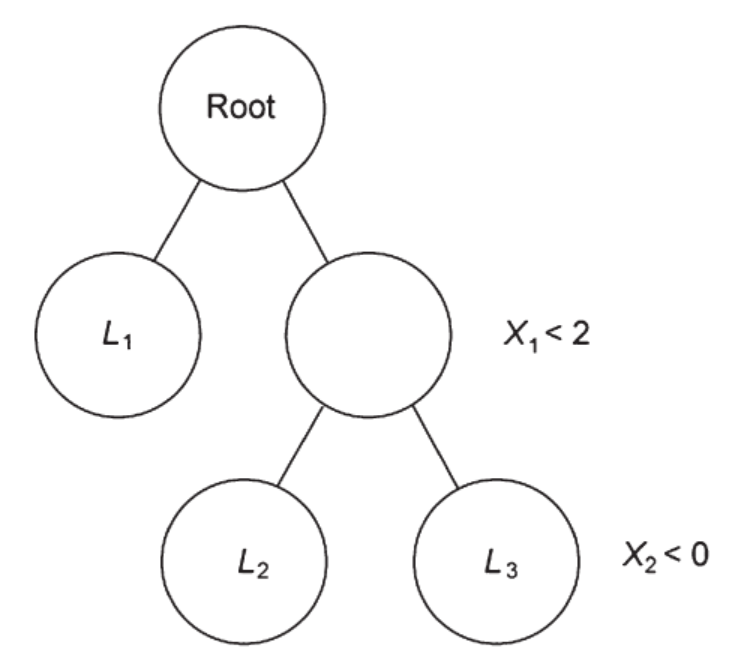
\includegraphics[width=0.6\linewidth]{tree.png}
        \end{tikzfigure}
        \vspace{1em}

        Disadvantages relative to parametric models:
        \begin{itemize}
            \item decreased efficiency when the parametric models are adequate
            \item discontinuities at partition boundaries
            \item categorical predictors with many levels can cause computational difficulties
        \end{itemize} 
    }

    \column{0.36}
    \block{3. Imputation algorithm}{
    
        Let $Y$ be $n \times p$ the data matrix arranged as $Y= (Y_p, Y_c)$, where
        \begin{itemize}
            \item $Y_p$ consists of $p_1$ \textit{partially observed} columns, such that moving from left to right, the number of missing elements in each column is nondecreasing
            \item  $Y_c$ remaining completely observed columns
            \item  $Y_{obs}$ set of observed and $Y_{mis}$ set of missing elements 
        \end{itemize}

        \vspace{10mm}



        4-steps algorithm:
        \begin{enumerate}
            \item Initial values for the missing values filled in as follows:
            \begin{enumerate}
                \item Define a matrix $Z$ equal to $Y_c$
                \item Impute missing values in $Y_i$, where $i=1, ... p_1$, using CART on $Z$ and append the completed version of $Y_i$ to $Z$ prior to incrementing $i$             
            \end{enumerate}       
            \item  Replace the originally missing values of $Y_i$, where $i=1, ... p_1$, with CART on $Y_{-i}$
            \item Repeat $l$ times step 2
            \item Repeat steps 1–3 $m$ times and obtain $m$ imputed sets.
        \end{enumerate}   


        \vspace{10mm}

  %      \begin{itemize}
  %          \item sequential CART imputation algorithm
  %          \item  order the variables from least amount to largest amount of missing data
  %          \item minimum leaf size of 5 and the splitting criteria of a deviance greater than 0.0001
  %          \item trees are not pruned to minimize bias
  %          \item size of trees modulated by requiring a minimum number of observations in each leaf and by %controlling the minimum heterogeneity in the values in the leaf in order to consider it for further splitting     
  %          \item We take draws from the predictive distribution by sampling elements from the leaf that corresponds to the covariate values of the record of interest
  %          \item  actually perform a Bayesian bootstrap within each leaf before sampling.
   %     \end{itemize}
 }

            \block{4. Comparison mice/miceRanger packages}{
        \begin{itemize}
            \item both implement Stef van Buuren’s Multivariate Imputation by Chained Equations
            \item \textit{mice} supports variety of imputation methods, \textit{miceRanger} only randomForest
            \item \textit{mice} uses common R packages “rpart” and “randomForest” to implement tree based imputation methods (van Buuren 2023)
            \item \textit{miceRanger} uses the “ranger”-package instead, which claims to be faster and more efficient with medium and large data sets (Wilson 2022)
                \begin{itemize}
                    \item[$\Rightarrow$] core functions written in C++ (faster than R, compiled vs. interpreted code) (Wright und Ziegler 2017)
                    \item[$\Rightarrow$] supports parallel computing (Wright und Ziegler 2017; Wright 2023)
                \end{itemize}
        \end{itemize}
    }
            \block{5. Empirical simulation study}{
            Objective:
            \begin{itemize}
            \item evaluate efficacy of tree-based imputation methods on missing data
            \item compare \textit{mice} package methods against the extended methods in \textit{miceRanger}
            \end{itemize} 
            
            Empirical data set:
            \begin{itemize}
            \item RAND's Health Insurance Experiment
            \end{itemize}

            Monte Carlo simulation:
            \begin{itemize}
                \item simulations (R): 1000 cycles to ensure robustness
                \item multiple imputations (M): 5 imputations to estimate variability
                \item sample size (n): 2000 cases to ensure generalizability.
  
            \end{itemize}
    }

    \column{0.32}
    \block{}{
    \begin{itemize}
        \item iterations (niter): 10 iterations for chained equations.
        \item random forest trees (nrtree): 10 trees in each RandomForest model for depth
    \end{itemize}
    Comparison Metrics: determine the most accurate and efficient imputation method that best reconstructs true values while minimizing systematic errors
    \begin{itemize}
        \item bias: deviation of imputed values from true values.
        \item mean squared error: average squared difference between the imputed and true values.
        \item coverage: proportion of times true values fall within the calculated confidence intervals.
    \end{itemize}
    
    }
   
    \block{6. Results}{

    

        \centering
        \begin{tabular}{|l|l|lll|}
             \hline   
             Metric &  Method & Bias \hspace{3mm} & MSE \hspace{3mm} & Coverage \hspace{3mm}\\
             \hline
             mean(age) & BD & NA & NA & NA\\
             mean(age) & CC & NA & NA & NA\\
             mean(age) & CART & NA & NA & NA\\
             mean(age) & RandomForest & NA & NA & NA\\
             mean(age) & miceRanger  & NA & NA & NA \\
             \hline
             mean(educ) & BD & NA & NA & NA\\
             mean(educ) & CC & NA & NA & NA\\
             mean(educ) & CART & NA & NA & NA\\
             mean(educ) & RandomForest & NA & NA & NA\\
             mean(educ) & miceRanger  & NA & NA & NA \\
             \hline
             $\rho$(mdvis, hltg)  & BD & NA & NA & NA\\
             $\rho$(mdvis, hltg) & CC & NA & NA & NA\\
             $\rho$(mdvis, hltg) & CART & NA & NA & NA\\
             $\rho$(mdvis, hltg) & RandomForest & NA & NA & NA\\
             $\rho$(mdvis, hltg) & miceRanger  & NA & NA & NA \\
             \hline
             reg.(mhi)  & BD & NA & NA & NA\\
             reg.(mhi) & CC & NA & NA & NA\\
             reg.(mhi) & CART & NA & NA & NA\\
             reg.(mhi) & RandomForest & NA & NA & NA\\
             reg.(mhi) & miceRanger  & NA & NA & NA \\
             \hline
        \end{tabular}
}




    


    }
    
    \block{7. Conclusion}{

    }
    \block{References}{
        \vspace{-1em}
        \begin{footnotesize}
        \printbibliography[heading=none]
        \end{footnotesize}
    }
\end{columns}
\end{document}